\documentclass{article}
\usepackage[T1]{fontenc}
\usepackage[ansinew ]{inputenc}
\usepackage{amsmath}
\usepackage{tikz}
\usepackage{tikzsymbols}
\usepackage{lmodern}
\usepackage{xcolor}
\usetikzlibrary{arrows,automata}
\setlength\parindent{0pt}

\begin{document}

\begin{center}
  \Large{Informatik D - �bungsblatt 4}

  \large{Sebastian H�ffner, Andrea Suckro}
\end{center}



\section{Aufgabe 4.1}
Automat zur Addition zweier bin\"arer Zahlen.
\begin{center}
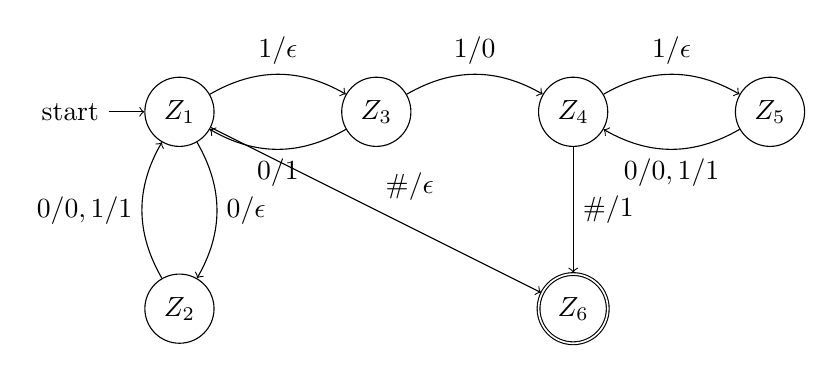
\begin{tikzpicture}[->, auto, node distance=2.5cm]
  \node[initial,state]   (Z1)               {$Z_1$};
  \node[state]           (Z2) [below of=Z1] {$Z_2$};
  \node[state]           (Z3) [right of=Z1] {$Z_3$};
	\node[state]           (Z4) [right of=Z3] {$Z_4$};
	\node[state]           (Z5) [right of=Z4] {$Z_5$};
  \node[state,accepting] (Z6) [below of=Z4] {$Z_6$};

  \path (Z1) edge [bend left]            node {$1/\epsilon$} (Z3)
             edge                        node {$\#/\epsilon$}(Z6)
						 edge [bend left]            node {$0/\epsilon$} (Z2)
        (Z2) edge [bend left]            node {$0/0,1/1$}    (Z1)
        (Z3) edge [bend left]            node {$0/1$}        (Z1)
             edge [bend left] 					 node {$1/0$}        (Z4)
				(Z4) edge [bend left]						 node {$1/\epsilon$} (Z5)
						 edge												 node {$\#/1$}			 (Z6)
				(Z5) edge [bend left]					   node {$0/0,1/1$}    (Z4)
        ;
\end{tikzpicture}
\end{center}


\section{Aufgabe 4.2}

\section{Aufgabe 4.3}

\section{Aufgabe 4.4}

\section{Aufgabe 4.5}

\section{Aufgabe 4.6}




\end{document}